\part{Part 1: Introduction to electrical machines and drives}
\title[Introduction]{Introduction to electrical machines and drives}  
\date{}  
\frame{\titlepage} 

%%%%%%%%%%%%%%%%%%%%%%%%%%%%%%%%%%%%%%%%%%%%%%%%%%%%%%%%%%%%%
%% What is an electrical machine ? %%
%%%%%%%%%%%%%%%%%%%%%%%%%%%%%%%%%%%%%%%%%%%%%%%%%%%%%%%%%%%%%
\begin{frame}
	\frametitle{What is an electrical machine ?}
	%devide slide into two columns
	\begin{columns}
		\begin{column}{0.5\textwidth}
			\begin{defi}{Electrical machine}{elec_machine}
			   An electrical machine is a device that \hl{converts electrical energy into  mechanical energy} or vice versa.
			\end{defi}
			\vspace{0.25cm}
			\begin{itemize}
				\item Electrical energy is routed via machine's external wiring connected to the terminal box.
				\item Mechanical energy is transferred via the shaft (if it is a rotatory machine).
			\end{itemize}
		\end{column}
		\begin{column}{0.5\textwidth}
			\begin{figure}
				\centering
				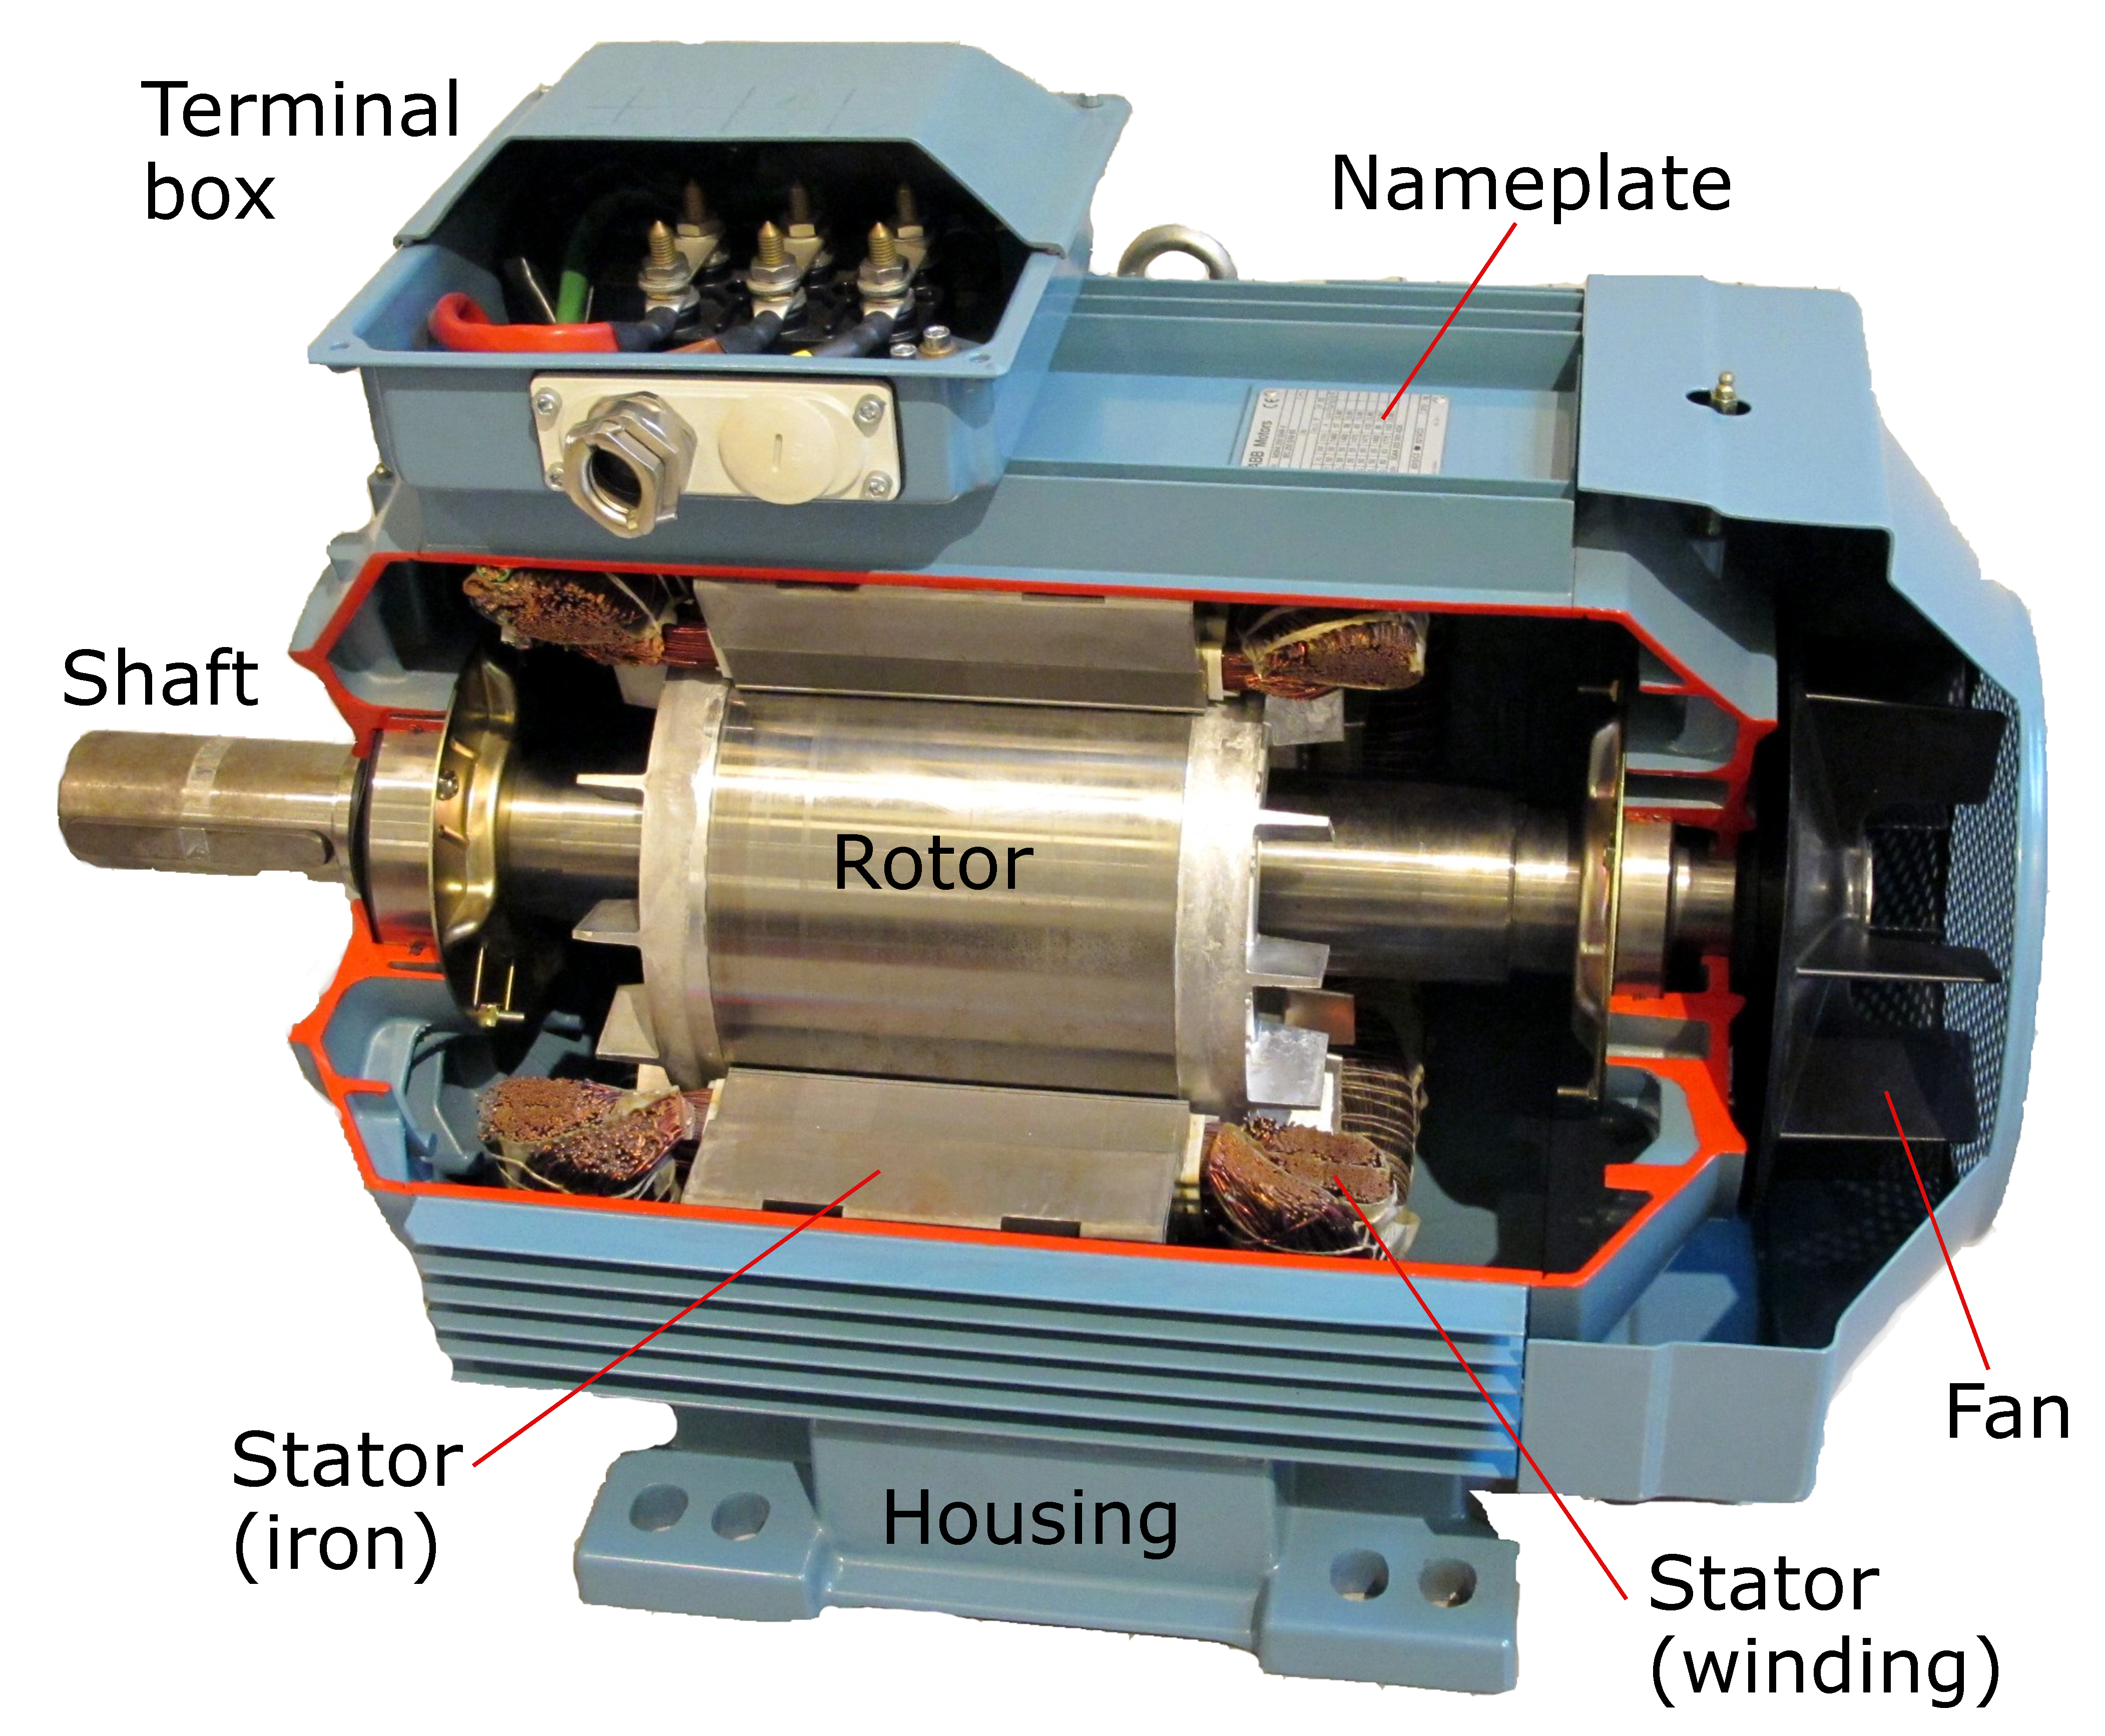
\includegraphics[width=0.95\textwidth]{fig/lec01/Induction_machine_opened.pdf}
				\caption{Example of an electrical machine (source: derived from \href{https://commons.wikimedia.org/wiki/File:TMW_50906_Schnittmodell_einer_Drehstrommaschine_(Asynchronmaschine).jpg}{Wikimedia Commons}, public domain)}
			\end{figure}
		\end{column}
		\end{columns}
\end{frame}


%%%%%%%%%%%%%%%%%%%%%%%%%%%%%%%%%%%%%%%%%%%%%%%%%%%%%%%%%%%%%
%% What is an electrical drive ? %%
%%%%%%%%%%%%%%%%%%%%%%%%%%%%%%%%%%%%%%%%%%%%%%%%%%%%%%%%%%%%%
\begin{frame}
	\frametitle{What is an electrical drive ?}
	%devide slide into two columns
	\begin{columns}
		\begin{column}{0.4\textwidth}
			\begin{defi}{Electrical drive}{elec_drive}
			   An electrical drive is a system that \hl{controls the torque, speed or position of an electrical machine} connected to some mechanical process.
			\end{defi}
			\vspace{0.25cm}
			\begin{itemize}
				\item Integrates the 'stupid' electrical machine into an 'intelligent' controlled system.
				\item The energy source and mechanical process ('load') are not part of the drive system.
			\end{itemize}
		\end{column}
		\begin{column}{0.6\textwidth}
			\begin{figure}
				\centering
				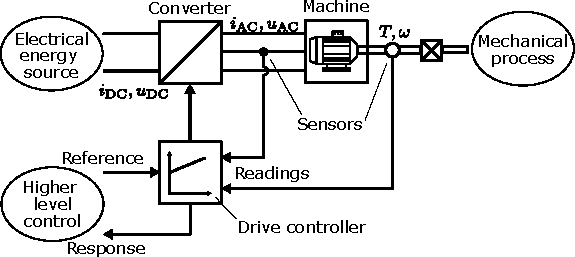
\includegraphics[width=0.95\textwidth]{fig/lec01/Electrical_Drive_Block_Overview.pdf}
				\caption{Block diagram of an electrical drive}
			\end{figure}
		\end{column}
	\end{columns}
\end{frame}